\section{Calcul d'erreurs}
\label{sec:erreurs}

Les erreurs sur les mesures sont données dans le \autoref{tab:erreurs}.

\begin{table}[h]
    \centering
    \begin{tabulary}{\textwidth}{C C}
        \toprule
        Variable & Erreur \\
        \midrule
        \(\Delta V_\textrm{min}\) [\si{\centi\meter\cubed}] & 30 \\
        \(\Delta V_\textrm{max}\) [\si{\centi\meter\cubed}] & 90 \\
        \(\Delta p_\textrm{min}\) [\si{\bar}] & 0.05 \\
        \(\Delta p_\textrm{max}\) [\si{\bar}] & 0.05 \\
        \(\Delta U_\textrm{fil}\) [\si{\volt}] & 0.05 \\
        \(\Delta I_\textrm{fil}\) [\si{\ampere}] & 0.05 \\
        \(\Delta T_\textrm{fil}\) [\si{\kelvin}] & 70 \\
        \(\Delta T_\textrm{eau}\) [\si{\kelvin}] & 0.1 \\
        \(\Delta D\) [\si{\milli\liter \per \minute}] & 5 \\
        \(\Delta C_\textrm{m,eau}\) [\si{\joule\per\kelvin\per\kilo\gram}] & 0.1 \\
        \(\Delta \rho_\textrm{eau}\) [\si{\kilo\gram\per\meter\cubed}] & 0.1 \\
        \(F\) [\si{\newton}] & 15\% \\
        \(\omega\) [\si{\radian \per \second}] & 5\% \\
        \bottomrule
    \end{tabulary}
    \caption{Erreurs estimées sur les mesures}
    \label{tab:erreurs}
\end{table}

\paragraph*{Regression linéaire}
Les erreurs sur les régressions linéaires \(y = ax + b\) sur les mesures \((x_i, y_i) ; i = \{1, \hdots, n\}\) sont donnés par l'équation \cite{erreursmesure}:

\begin{equation}
    \label{eq:erreur:fit}
    \begin{aligned}
        (\Delta a)^2 &= \frac{\sum_{i=1}^{n}(y_i - (a x_i + b))^2}{(n-2) \sum_{i=1}^{n}(x_i - \bar{x})^2}\\
        \Delta b &= \bar{x} \Delta a + a \Delta \bar{x}
    \end{aligned}
\end{equation}

En pratique, ces valeurs sont calculées par la bilbiothèque python \texttt{numpy}.

\paragraph*{Formules d'erreurs}

Erreur sur le rendement théorique
\begin{equation}
    \Delta \eta = \eta \left( \left|\frac{\Delta T_1}{T_1}\right| + \left|\frac{\Delta T_2}{T_2}\right| \right)
\end{equation}

Erreurs sur les flux
\begin{equation}
    \Delta \phi_1 = \phi_1 \left( \left|\frac{\Delta (\Delta T)}{(\Delta T)}\right| + \left|\frac{\Delta D}{D}\right| \right), 
    \Delta \phi_2 = \phi_1 \left( \left|\frac{\Delta U}{U}\right| + \left|\frac{\Delta I}{I}\right| \right)
\end{equation}

Erreurs sur les puissance de différentes méthodes
\begin{align}
    \Delta P_\textrm{m,PV} &= P_\textrm{m,PV} \left( \left|\frac{\Delta c}{c}\right| + \left|\frac{\Delta A}{A}\right| + \left|\frac{\Delta \omega}{\omega}\right| \right)\\
    % \\
    \Delta P_\textrm{m,frein} &= P_\textrm{m,frein} \left( \left|\frac{\Delta F}{F}\right| + \left|\frac{\Delta \omega}{\omega}\right| \right)\\
    % \\
    \Delta P_\textrm{m,chaleur} &= P_\textrm{m,chaleur} (|\Delta \phi_1| + |\Delta \phi_2|)
\end{align}

Erreur sur le rendement expérimental 
\begin{equation}
    \Delta \eta = \eta \left( \left|\frac{\Delta P_m}{P_m}\right| + \left|\frac{\Delta \phi_2}{\phi_2}\right| \right)
\end{equation}

Toutes ces erreurs sont calculées en pratique par la bibliothèque \texttt{uncertainties}.

\section{Images}
\label{sec:image}

\begin{figure}[h]
    \centering
    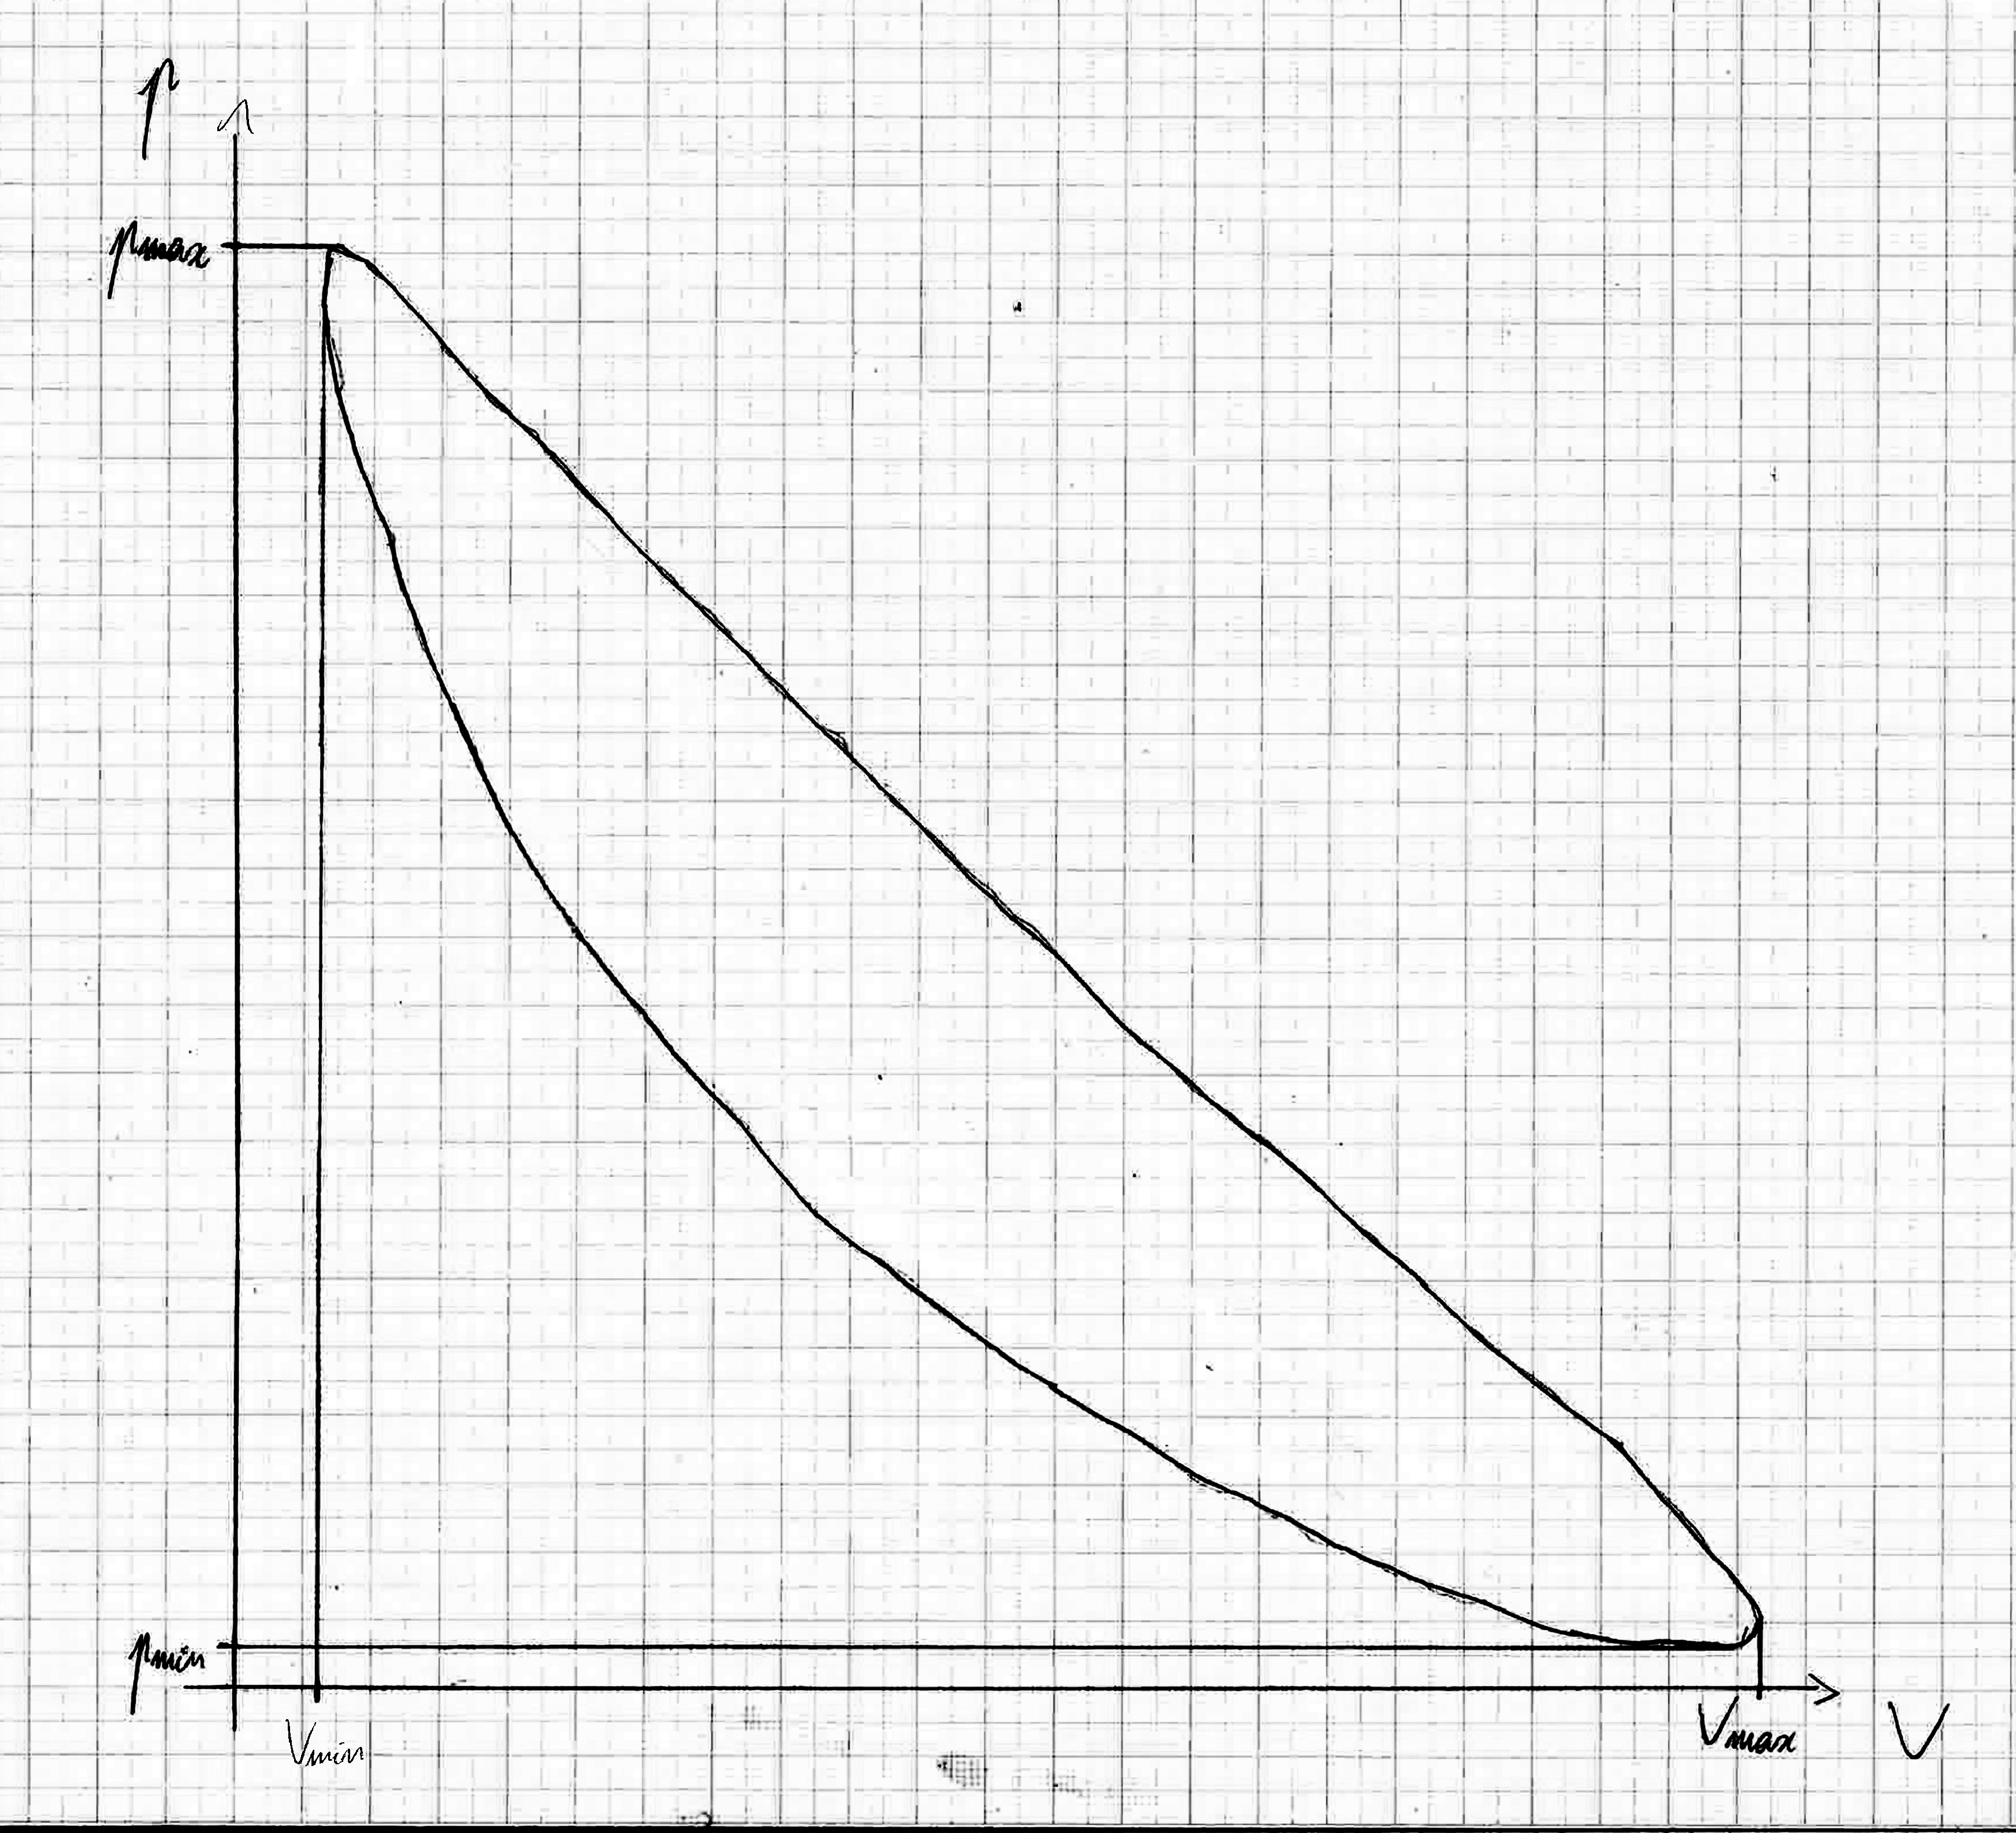
\includegraphics[width=\linewidth]{figures/scan_graph.png}
    \caption{Diagramme PV du moteur de Stirling}
    \label{fig:diag_pv}
\end{figure}

%% Haha shitpost go brr
\textcolor{white}{le jeu (t'as perdu)}
